% !TEX TS-program = LuaLaTeX
% !TEX encoding = UTF-8 Unicode
%! program = pdflatex
\documentclass[12pt,a4paper]{memoir} % for a long document

\renewcommand\printtoctitle[1]{\huge\bfseries #1}
\chapterstyle{dash}

%\documentclass[12pt,a4paper,article]{memoir} % for a short document
%\documentclass{report}
\usepackage{fontspec}
\usepackage{amsmath}
\usepackage{amsfonts}
\setmainfont{Arial}
%\setmainfont[Ligatures=TeX]{TeX Gyre Bonum}
%\setsansfont[Ligatures=TeX,Scale=MatchLowercase]{Latin Modern Sans}
%\setmonofont[Scale=MatchLowercase]{Menlo}
\linespread{1.1}% spread lines out a little
\frenchspacing % remove extra space after punctuation

\renewcommand{\contentsname}{Table des matières}
\renewcommand{\chaptername}{Chapitre}
\renewcommand{\bibname}{Bibliographie}
\renewcommand\listfigurename{Liste des figures}
\renewcommand\listtablename{Liste des tables}

\begin{document}
\title{BM3D sur GPU "Image denoising by sparse 3D transform-domain collaborative filtering"}
\author{\small{Stéphane Cuenat}}
\date{\small{30 janvier 2016}}
\maketitle

\begin{abstract}
Dans ce papier nous proposons une implementation open-source (C++/Cuda) de l'algorithme BM3D porté sur GPU. Nous discutons du choix de l'ensemble des paramètres et de l'influence de ceux-ci sur l'algorithme. Chaque phase (estimation basic \& estimation finale) est étudié séparément afin d'obtenir la meilleure qualité et vitesse de l'algorithme. Nous démontrons que BM3D est parallélisable, donc exécutable dans un monde GPU.   

\end{abstract}

\newpage

\tableofcontents

% !TEX TS-program = LuaLaTeX
% !TEX encoding = UTF-8 Unicode

\chapter{Introduction}
\paragraph{}
\textit{Collaborate Filtering} est le nom de la méthode the groupage et de filtrage de l'algorithme BM3D. Cette méthode est réalisée en 4 étapes: 1) Trouver a bloc (portion de l'image) similaire à un bloc de référence et ensuite grouper les ensemble pour former un bloc 3D. 2) Appliquer une transformée 3D sur l'ensemble des bloc 3D. 3) Réduire les coefficient du monde spectrale. 4) Appliquer la transformée 3D inverse. 
\paragraph{}
En atténuant le bruit, le \textit{Collaborate Filtering} révèle les plus petits détails partagés par les groupes de blocs. Chaque bloc filtré est alors remit à sa position d'origine. Sachant que deux blocs peuvent se chevaucher, nous pouvons obtenir plusieurs estimations pour un pixel donné. C'est pourquoi, nous devons les combiner. Cette étape finale est l'\textit{Aggrégation}.
\paragraph{}
Le premier filtre collaboratif est considérablement amélioré par un second filtre \textit{Wiener Filtering}. Cette seconde étape mime la premières étapes avec deux différences. Le \textit{Block-Matching} est appliqué sur l'image filtré et non sur l'image bruité. Nous n'appliquons plus un filtre \textit{Hardthreshold} mais un filtre \textit{Wiener Filtering}. L'étape finale d'\textit{Aggrégation} reste inchangée.
\paragraph{}
L'algorithme BM3D détaillé ici est directement tiré de l'article originale \cite{1}. Plusieurs analyses préalable de l'algorithme BM3D démontre une diminution de la performance de débrouillage lorsque la déviation standard du bruit dépasse 40. Il a été démontré que pour de grande valeurs de bruit (standard deviation), les paramètres doivent être revu. Le seuil de filtrage de la première phase doit être augmenté. Il a aussi été démontré que les transformées 2D appliquées peuvent influencer l'algorithme. Dans \cite{2}, ils montrent que la meilleurs qualité d'image est atteinte en appliquant une transformée \textit{2D bi-orthogonal spline wavelet}. 
\paragraph{}
Dans ce papier nous nous sommes focaliser sur la qualité, mais plus particulièrement sur l'implémentation sur GPU (parallélisation de l'algorithme BM3D). Pour une question de simplicité, nous avons décidé d'appliquer des DCT-2D (même si nous savons que nous pouvons atteindre une meilleure qualité en appliquant d'autres transformées lors de la phase 1 et 2). Nous allons montrer dans les chapitres suivants que nous avons une bonne qualité en comparaison à \cite{3}. Pour ce qui est de la transformé 1D selon Z, nous avons opté pour la transformée d'Hadamar-Welsh \cite{4}. Nous verrons que cette méthode est efficace sur GPU. Dans \cite{1}, l'algorithme (écrit avec Matlab) est capable de traiter une image en 4 secondes. Ce temps est relativement long. Le but de ce papier est  de montrer que nous pouvons profiter de la puissance du GPU pour  réduire ce temps à quelques milisecondes, ce qui revient à montrer que BM3D peut être paraléliser.   
\paragraph{}
Dans le chapitre 2, nous présentons en détails l'algorithme BM3D. Le chapitre 3 est dédié à la réalisation sur GPU. Au chapitre 4, nous présentons nos résultats obtenus en comparaison aux travaux menés par \cite{3}. Nous présentons nos conclusions et les prochaines étapes au chapitre  5.     
% !TEX TS-program = LuaLaTeX
% !TEX encoding = UTF-8 Unicode

\chapter{Algorithme BM3D}
%-------------------------------------------General-----------------------------------
\section{Concept général}
Dans ce chapitre nous allons présenter les différentes étapes de l'algorithme BM3D sur des images de niveau de gris. Concernant l'application de l'algorithme sur des images couleurs, vous trouverez une explication dans \cite{2}. Dans la suite, nous assumons que le bruit est un bruit Gaussien et sa variance est equal à \(\sigma^2\) (\sigma \: étant la déviation standard du bruit appliqué sur l'image originale).
\newline
\newline
L'algorithme est divisé en deux étapes:
\newline
\newline
\begin{enumerate}
\item La première étape consiste à estimer le bruit par "hard thresholding" lors du filtrage collaboratif. Les paramètres de cette étapes sont représentés par l'exposant \textbf{hard}.
\item La deuxième étage est basée sur l'image bruité et sur l'estimation issue de la première étape. Cette étape utilise un filtre "Wiener Filter" lors du filtrage collaboratif. Les paramètres liés à cette étape sont représentés à l'aide de l'exposant \textbf{wiener}.
\end{enumerate}
\newpage
\begin{figure}[h]    
    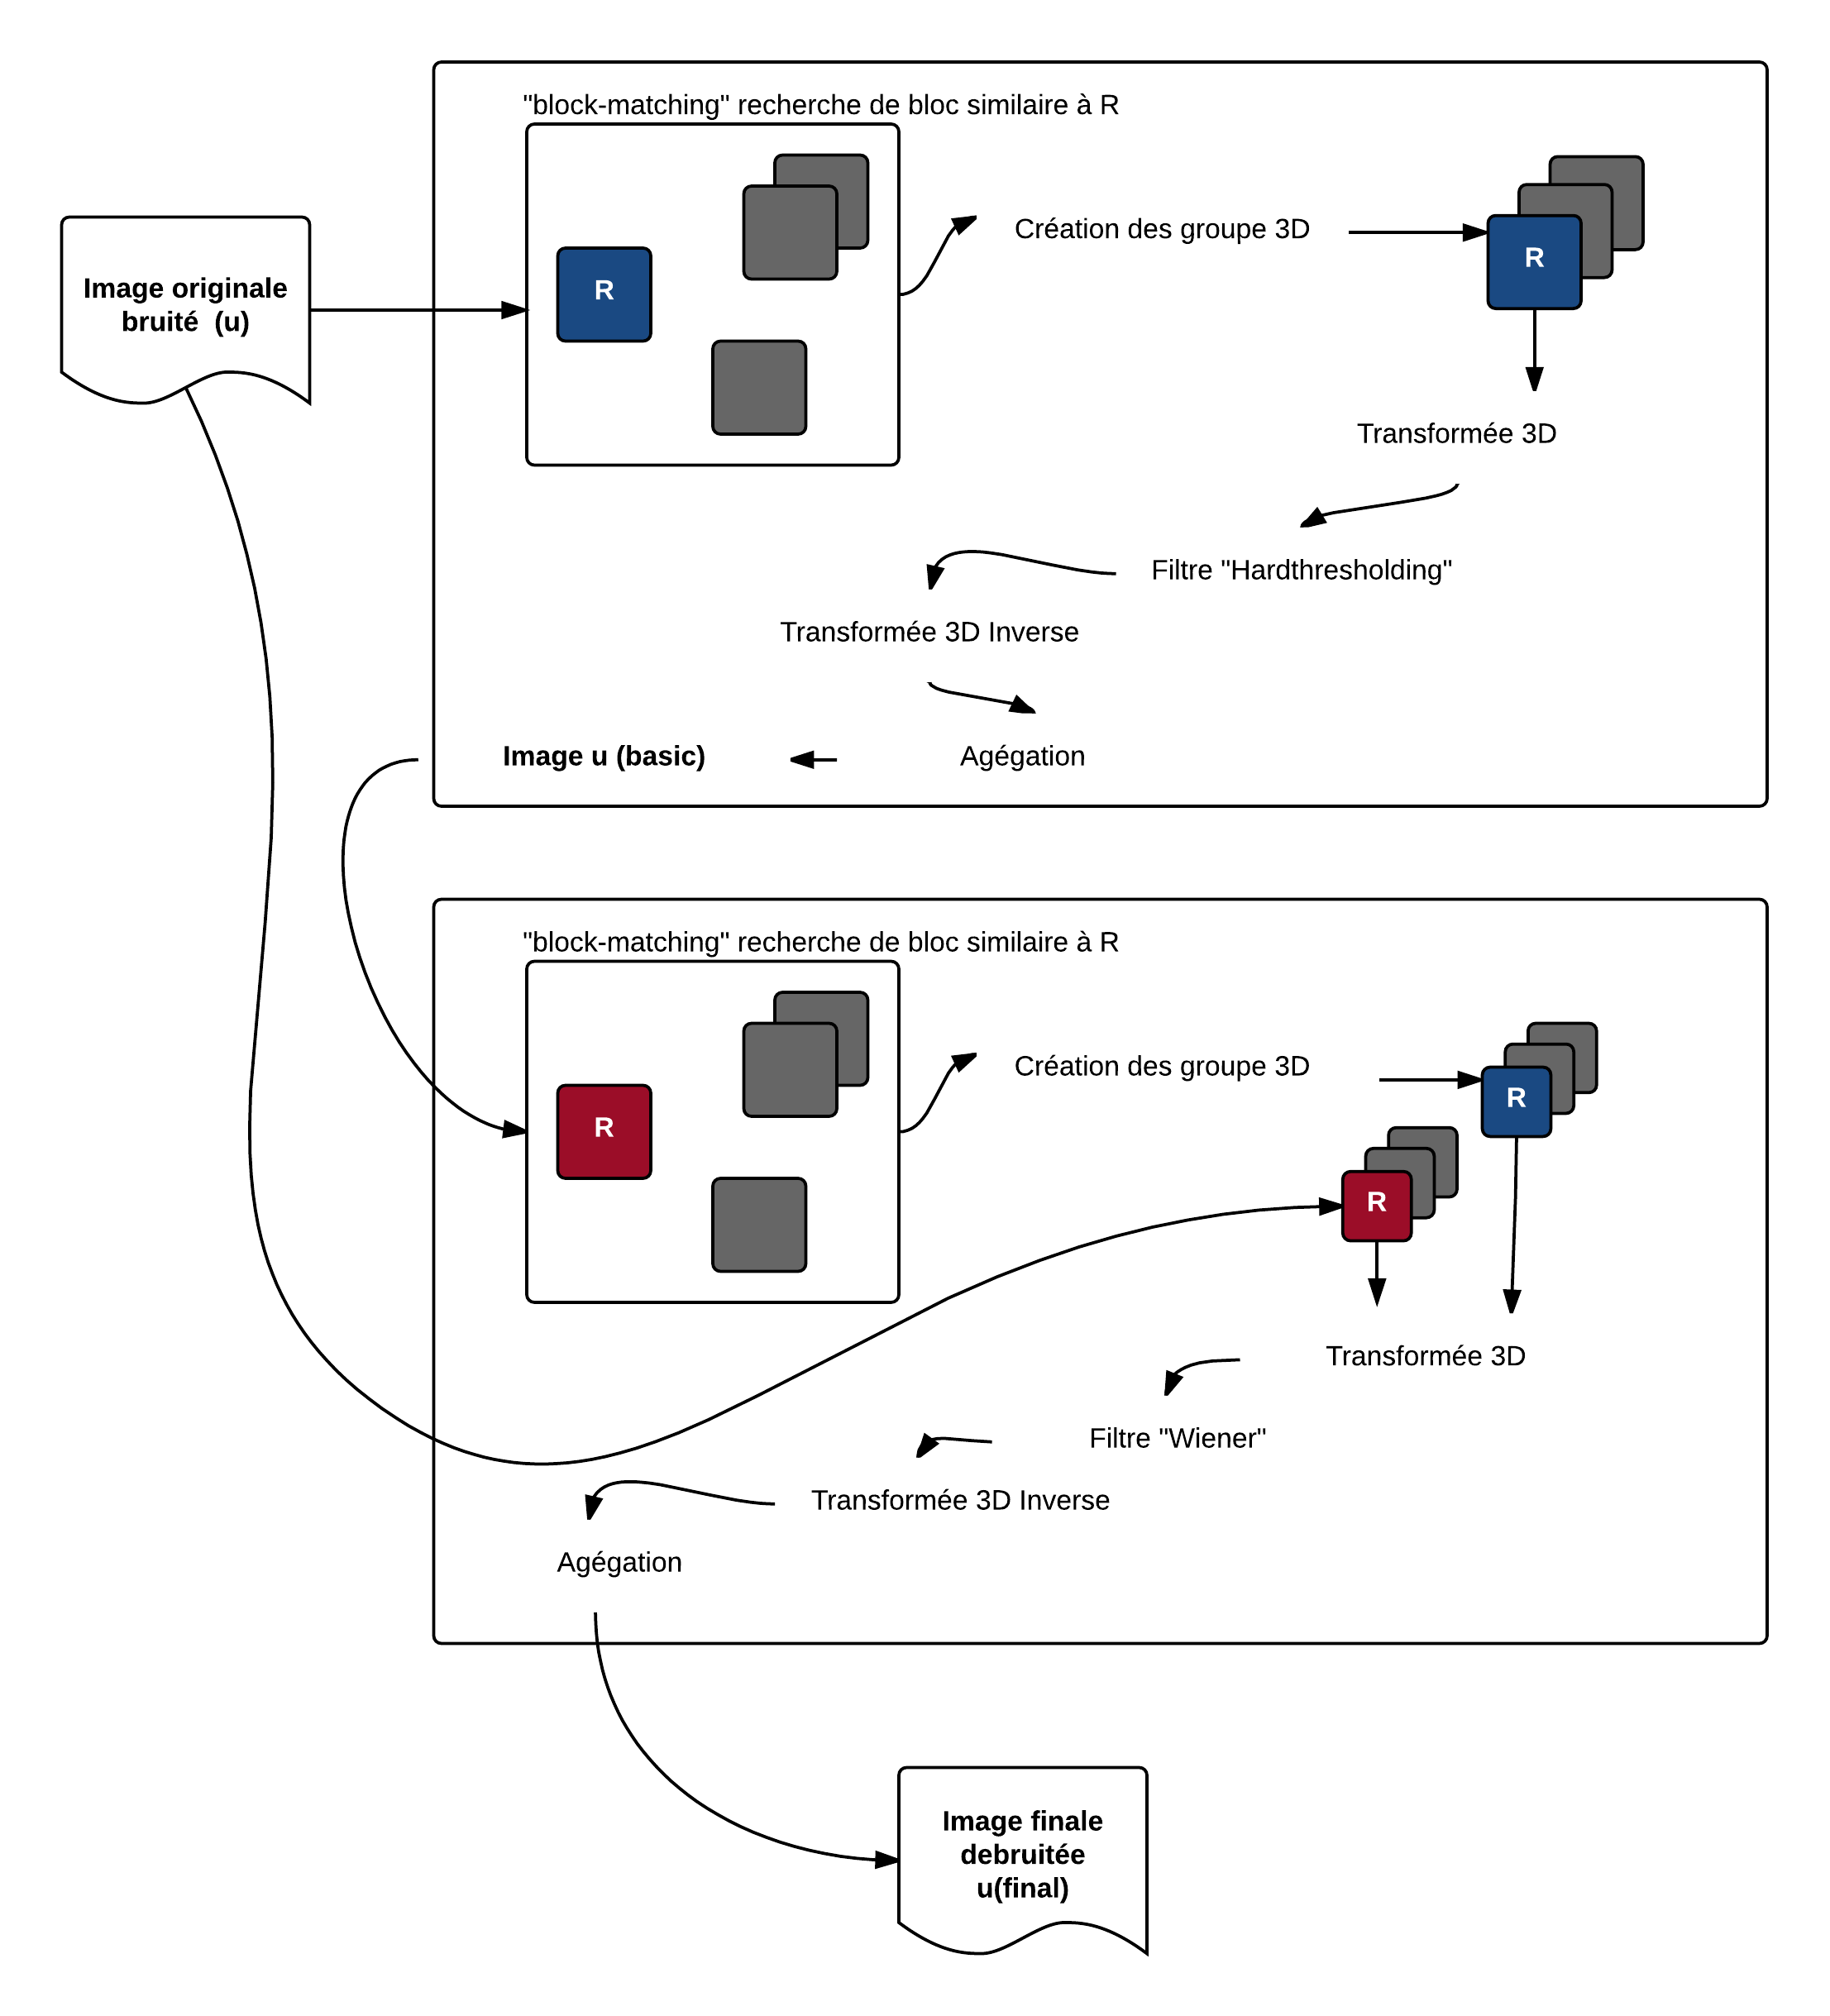
\includegraphics[scale=0.8]{algo}
    \caption{L'algorithme BM3D}
\end{figure}
\newpage

%-------------------------------------------Basic estimate-----------------------------------
\section{Estimation basic (phase 1)}
On dénote par P le bloc (bloc) de référence de taille \(K^{hard} * K^{hard}\).
\begin{figure}[h]    
    \centering
    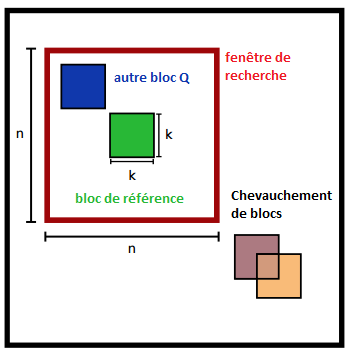
\includegraphics{bloc}
    \caption{blocs, fenêtre de recherche et chevauchement}
\end{figure}

\subsection{Groupement ("Block matching")}
Cette première sous-étape regroupe l'ensemble des blocs similaires à chaque bloc de référence P. Pour chaque bloc de référence P, on recherche les blocs Q similaire à P dans une fenêtre centrée sur P de taille \(n^{hard} * n^{hard}\). Le groupe de blocs est défini par: 
\begin{equation}
P(P) = \{Q: d(P,Q) \leq \tau^{hard}\}
\end{equation}
\newpage
Ou
\begin{itemize}
\item \( \tau^{hard} \): est la distance limite pour laquelle deux blocs sont considérés comme similaire.
\item \(d(P,Q) = \frac{\parallel \gamma' (P) - \gamma'(Q) \parallel_2^2}{(k^{hard})^2} \) est la distance quadratique normalisée entre deux blocs\footnote{Nous avons ici calculé la distance Euclidienne carrée.}.
\item \gamma' est le seuil du filtre qui est equal à \(\lambda^{hard}_{2D}\sigma \). Pour un \sigma \leq 40, le seuil est equal à \(\lambda^{hard}_{2D}\sigma \) = 0. Pour \sigma \leq 40, tous les coefficients sont inchangés\footnote{Nous verrons au chapitre 3 (Réalisation) que nous avons omis cette étape ayant pris en compte des images avec un \sigma \leq 30 pour nos tests.}.  
\item \(\sigma^2\) \: est la variance du bruit Gaussien appliquée à l'image.
\end{itemize}

Le groupe 3D représenté par \(P \)(P) est construit en regroupant les blocs similaire \(P \)(P). Pour augmenter la performance de l'algorithme, seulement les \(N^{hard} \) blocs de \(P \)(P) qui sont les plus proches du bloc de référence P sont gardé pour formé le groupe 3D\footnote{Au chapitre 3 nous verrons que \(N^{hard} \) doit être une puissance de 2.}. L'ordre des blocs dans le groupe 3D n'a aucune influence sur le résultat. Ceux-ci peuvent être désordonnés. 
\newpage
\subsection{Filtre collaboratif}
Une fois les groupe 3D construit, le filtre collaboratif est appliqué. On applique une transformée linéaire selon Z (profondeur du groupe 3D). Cette étape est suivie par un seuillage des coefficients du domaine spectrale. Pour finir nous appliquons une transformée 3D inverse afin de connaître l'estimation pour chaque bloc du groupe. 
\begin{equation}
\mathbb{P}(P)^{hard} = \tau^{hard^-1}_{3D} (\gamma (\tau^{hard}_{3D}(\mathbb{P}(P))))
\end{equation}
Ou \gamma \: est l'opérateur de seuil avec une limite \(\lambda^{hard}_{3D}\sigma\):
\[ \gamma(x) =
  \begin{cases}
    0       & \quad \text{si} \: x  \leq \lambda^{hard}_{3D}\sigma \\
    x       & \quad \text{sinon}\\
  \end{cases}
\]
Pour une raison pratique que nous démontrerons dans les prochains chapitres, la transformée 3D \(\tau^{hard}_{3D}\) du groupe 3D P(P) est effectuée en deux étapes. Nous appliquons une première transformée 2D dénoté \(\tau^{hard}_{2D}\)sur chaque bloc. Ensuite une transformée 1D dénoté par \(\tau^{hard}_{1D}\) est appliquée sur la troisième dimension du groupe 3D (profondeur).  

\subsection{Agrégation}
La dernière étape est l'agrégation. Nous avons une estimation pour chaque bloc et donc une estimation pour chaque pixel. Ces estimations sont sauvegardées dans deux zones tampons ainsi définis:
\[ \forall Q \in  P(P), \forall x \in Q, 
  \begin{cases}
    v(x) = v(x) + w^{hard}_P u^{hard}_{Q,P}(x) \\
    \delta(x) = \delta(x) + w^{hard}_P  \\
  \end{cases}
\]
Ou:
\begin{itemize}
\item \(v (resp. \: \delta ) \) représente le numérateur (resp. le dénominateur) de l'estimation basic de l'image obtenue à la fin de l'étape de groupage.
\item \(u^{hard}_{Q,P} \) est l'estimation du pxiel \(x \) qui appartient au bloc Q obtenu lors de la phase du filtre collaboratif du bloc P.
\item \( w^{hard}_P  = \begin{cases} (N^{hard}_P)^{-1}  & \quad \text{si} \: N^{hard}_P \ge 1 \\ 1  & \quad\text{sinon}\\ \end{cases} \) 
\item \( N^{hard}_P \) correspond aux nombres de coefficients (non-zero) du bloc 3D après filtrage: \(\gamma ( \tau^{hard}_{3D} (\mathbb{P}(P))) \). 
\end{itemize}
\newpage
L'intérêt de cet méthode est qu'elle donne aux blocs homogènes (ou beaucoup de coefficient ont été éliminés) la priorité. Un bloc avec des effets de bords sera moins pris en compte que des blocs homogènes. La figure ci-dessous montre cette effet. L'algorithme donne plus d'importance aux blocs vert durant la phase d'agrégation.
\begin{figure}[h]    
    \centering
    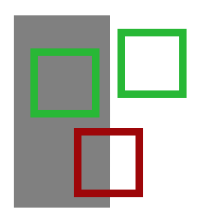
\includegraphics{chevauchement}
    \caption{Chevauchement de blocs}
\end{figure}
\newline
\newline
Afin de réduire les effets de bords qui peuvent apparaître, nous appliquons une Kaiser window (\( k^{hard} * k^{hard}\)) après la transformée 3D inverse sur chaque bloc. Cela revient à multiplier chaque coefficient de la Kaiser window avec le coefficient du bloc \footnote{Nous montrerons au chapitre 4 (Résultat) que cette étape influence peu le résultat final comme mentionné dans \cite{2}.}.  
\newline 
\newline
L'estimation basic obtenue après cette première étape est donnée par:
\begin{equation}
u^{basic}(x) = \frac{\displaystyle\sum_{P}w^{hard}_P \displaystyle\sum_{Q \in P(P)}X_Q(x)u^{hard}_{Q,P}(x)}{\displaystyle\sum_{P}w^{hard}_P \displaystyle\sum_{Q \in P(P)}X_Q(x)}
\end{equation}
\newpage
Avec \(X_Q(x)\) définit ainsi:
\[ X_Q(x) =
  \begin{cases}
    1       & \quad \text{si et seulement si} \: x  \in Q \\
    0       & \quad \text{sinon}\\
  \end{cases}
\]
Ce résultat est simplement obtenue en divisant les deux buffers préalablement calculés pour chaque pixel de l'image original: 
\begin{equation}
u^{basic}(x) = \frac{v(x)}{\delta(x)}
\end{equation}
\newpage

%-------------------------------------------Final estimate-----------------------------------
\section{Estimation finale (phase 2)}
Dans cette deuxième partie de l'algorithme, l'estimation basic \(u^{basic} \) issue de la première partie est accessible. Cette seconde étape applique un filtre \textit{Wiener Filter} sur l'image originale \(u \). Cette étape finale permet de restaurer plus de détails. 
\subsection{Groupement ("Block matching")}
Le regroupement des blocs (calcul de la distance entre blocs) est effectué sur l'estimation basic issue de la première partie de l'algorithme. Le groupe de blocs similaire est définit par:
\begin{equation}
P^{basic}(P) = \{ Q: d(P,Q) \leq \tau^{wien} \}
\end{equation}
Deux 3D groupes sont formé:
 \begin{enumerate}
\item \(\mathbb{P}^{basic}(P) \) en regroupant les blocs similaires  depuis l'image issue de l'estimation basic \(u^{basic}\).
\item \(\mathbb{P}(P)\) en regroupant les blocs de la même manière qu'au point 1 depuis l'image bruité originale \(u\).
\end{enumerate}
Pour une question d'optimisation de l'algorithme, seul \(N^{wien} \) blocs sont pris en comptes pour chacun des 3D groupes\footnote{Nous verrons que \(N^{wien} \) doit être une puissance de 2 comme \(N^{hard} \) lors de la phase 1 (estimation basic).}.
\subsection{Filtre collaboratif}
Lorsque les groupe 3D sont formés, le filtre collaboratif peut être appliqué. Pour cela, les \textit{Wiener} coefficients sont definis par:
\begin{equation}
w_P(\xi) = \frac{\mid \tau^{wien}_{3D} (\mathbb{P}^{basic}(P))(\xi) \mid^2}{\mid \tau^{wien}_{3D}(\mathbb{P}^{basic}(P))(\xi) \mid^2 + \sigma^2}
\end{equation}
\newpage
Le filtre collaboratif \textit{Wiener} de \(\mathbb{P}(P)\) est réalisé par la multiplication élément par élément de la transformée 3D de l'image bruité avec les coefficients \textit{Wiener} \(w_P\). Lors de cette étape, l'estimation d'un groupe 3D est ainsi obtenu:
\begin{equation}
\mathbb{P}^{wien}(P) = \tau_{3D}^{wien^{-1}} (w_P * \tau_{3D}^{wien}(\mathbb{P}(P)))
\end{equation}
\subsection{Agrégation}
L'agrégation est basé sur les même concepts décrit lors de la première phase de l'algorithme. Les estimations de chaque pixel seront maintenu dans deux zones tampons définis par:
\[ \forall Q \in  P(P), \forall x \in Q, 
  \begin{cases}
    v(x) = v(x) + w^{wien}_P u^{wien}_{Q,P}(x) \\
    \delta(x) = \delta(x) + w^{wien}_P  \\
  \end{cases}
\]
Ou:
\begin{itemize}
\item \(v (resp. \: \delta ) \) représente le numérateur (resp. le dénominateur) de l'estimation finale de l'image obtenue à la fin de l'étape de groupage.
\item \(u^{wien}_{Q,P} \) est l'estimation du pxiel \(x \) qui appartient au bloc Q obtenu lors de la phase du filtre collaboratif du bloc P.
\item \( w^{wien}_P  = \parallel w_P \parallel^{-2}_2 \). 
\end{itemize}
Comme lors de la première étape de l'algorithme, une Kaiser window \(k^{wien} * k^{wien}\) est appliqué pour réduire les effets de bords. L'estimation finale est donnée par:
\begin{equation}
u^{finale}(x) = \frac{\displaystyle\sum_{P}w^{wien}_P \displaystyle\sum_{Q \in P(P)}X_Q(x)u^{wien}_{Q,P}(x)}{\displaystyle\sum_{P}w^{wien}_P \displaystyle\sum_{Q \in P(P)}X_Q(x)}
\end{equation}
Avec \(X_Q(x)\) définit ainsi:
\[ X_Q(x) =
  \begin{cases}
    1       & \quad \text{si et seulement si} \: x  \in Q \\
    0       & \quad \text{sinon}\\
  \end{cases}
\]
L'estimation finale peut être obtenu de la même manière que l'estimation basic, en calculant (2.4) pour chaque pixel de l'image originale \(u\) \footnote{la création de deux zones tampons est approprié à l'exécution sur GPU, comme nous allons le montrer dans les prochains chapitres.}. 
% !TEX TS-program = LuaLaTeX
% !TEX encoding = UTF-8 Unicode

\chapter{Réalisation}
\section{Block matching}
\subsection{Calul de la distance euclidienne}
\subsection{Tri des blocks}
\section{"3D transfom"}
\section{Filtre "Hardthreshold"}
\section{Filtre de "Wien"}
\section{Aggregation}

% !TEX TS-program = LuaLaTeX
% !TEX encoding = UTF-8 Unicode

\chapter{Résulats}
\section{BM3D vs BM3D-GPU}
\section{Influance de la taille de la fenêtre de recherche}
\section{Influance de la Kaiser-Window}
\section{Influance de la transformée 2D sur les blocks avant "Block-Matching"}
\section{Influance du calcul de distance sur la rapidité de l'algorithme}
\section{Influance du tri des block sur la rapidité de l'algorithme}

% !TEX TS-program = LuaLaTeX
% !TEX encoding = UTF-8 Unicode

\chapter{Conclusion}
\section{Block matching}

\begin{appendix}
  \listoffigures
  %\listoftables
\end{appendix}

\bibliographystyle{plain}
\bibliography{biblio.bib}

\end{document}